\section{Software Design Patterns}

\begin{frame}
  \frametitle{Brief History}
  \begin{itemize}
    \item{Architecture: Christopher Alexander 1977/79}
      \begin{itemize}
        \item{A Place To Wait}
      \end{itemize}\pause{}
    \item{Beck \& Cunningham 1987}\pause{}
    \item{GoF Patterns (Gamma et al.) 1994}\pause{}
    \item{Many more since then}
  \end{itemize}
\end{frame}

\begin{frame}
  \frametitle{What Are Patterns}
  \begin{itemize}
    \item{Solutions to common problems}
    \item{NOT code}\pause{}
    \item{Descriptions of relevant forces}\pause{}
    \item{Language independent}
  \end{itemize}
\end{frame}

\begin{frame}
  \frametitle{Misconceptions}
  \begin{itemize}
    \item{Patterns are invented}\pause{}
    \item{GoF patterns are the only patterns}\pause{}
    \item{More patterns == Better software}\pause{}
    \item{Patterns have no drawbacks}\pause{}
    \item{Singleton is a good pattern}
  \end{itemize}
\end{frame}

\begin{frame}
  \frametitle{Pattern Sources}
  \begin{itemize}
    \item{GoF}\pause{}
    \item{POSA 1, 2, 3, 4}\pause{}
    \item{Security Patterns}\pause{}
    \item{Patterns for Fault Tolerant Software}\pause{}
    \item{Game Programming Patterns}\pause{}
    \item{Many, many more}
  \end{itemize}
\end{frame}

\begin{frame}
  \frametitle{Two Patterns for Asynchronous I/O}
  \begin{itemize}
    \item{Reactor}\pause{}
      \begin{itemize}
        \item{Notify when I/O is ready}
        \item{``Consumer'' must perform I/O}
      \end{itemize}\pause{}
    \item{Proactor}\pause{}
      \begin{itemize}
        \item{Notify when I/O is done}
        \item{``Consumer'' works with data}
      \end{itemize}\pause{}
  \end{itemize}
\end{frame}

\begin{frame}
  \frametitle{Proactor Relations}
  \vfill{}
  \begin{center}
    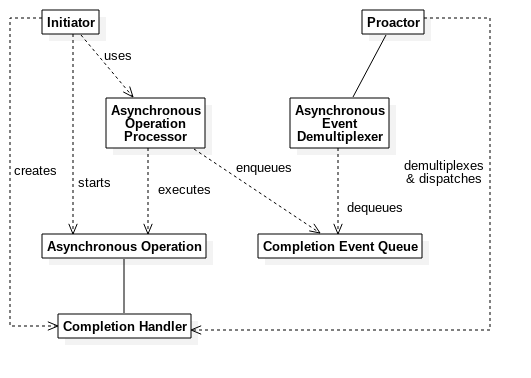
\includegraphics[width=0.8\textwidth]{proactor}
  \end{center}
\end{frame}
